%!TEX root = ../dissertation.tex
\chapter*{Preface}
\label{introduction}

Dear Reader! 

I am glad you are reading this dissertation.  

Writing the thesis is not an easy task. I have to summarize six years of my professional life into about two hundred pages, so let me start by presenting my Ph.D. project scope.  Be aware that the preface section contains several expressions that are not explicitly explained. You will find the discussion of the majority of them in the rest of this thesis.  I put much effort into making this thesis as clear and understandable as possible. 

All of my activities during the doctoral studies were related to one of four biggest, currently operating experiments at The European Organization for Nuclear Research CERN (fr.  Organisation européenne pour la recherche nucléaire).  It is called LHCb, and it stands for the Large Hadron Collider beauty experiment. The crucial part of the experiment is the LHCb detector, shown in figure \ref{fig:LHCBphoto}. Since there is not much to see besides the supporting steel structures, I also added a schematic cross-section of the experimental setup in figure \ref{fig:fig:LHCBlayout}. Each of the components, also called sub-detector, is described in chapter \ref{chapter:detector}. 


\begin{figure}[!hb]
\centering
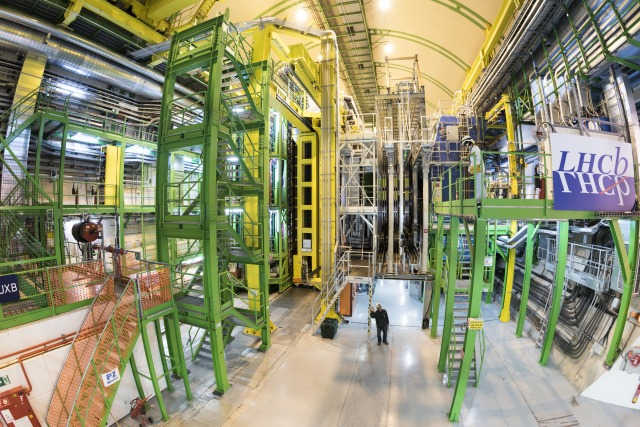
\includegraphics[width=\textwidth]{figures/LHCB_photo}
\caption{View of the detector LHCb. The image was taken from the CERN public website. 
\label{fig:LHCBphoto}}
\end{figure}

\begin{figure}
\centering
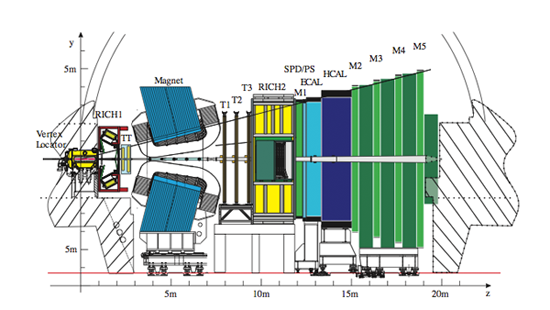
\includegraphics[scale=0.6]{figures/lhcblayout.png}
\caption{Layout of the LHCb detector, viewed from the side. The LHCb detector components from left to right: proton-proton interaction point, Vertex Locator Velo, Ring Imaging Cherenkov detector one (RICH1), TT, Magnet, T stations, RICH2, electromagnetic and hadrinic calorimeter (ECAL and HCAL), and muon stations. Figure taken from \cite{lhcb}. 
\label{fig:LHCBlayout}}
\end{figure}



From the physics point of view, the LHCb physics program is primarily focused on studying $CP$ violation, and rare phenomena in B (beauty) and C (charm) meson decays and searching for New Physics. Chapter \ref{chapter:physics} is dedicated to providing a brief description of the physics behind the LHCb experiment.  
The high-quality physics results obtained during the LHC Run I and Run II, proved excellent performance of the detector.
The list of outstanding physics results published by the LHCb Collaboration is extraordinary. For instance, LHCb collaboration was able to measure the very rare processes, such as $B_0\rightarrow \mu \mu$, occurring for once for every ten billion $B_0$ mesons \cite{B_mumu}, and the very first measurement of pentaquark state \cite{pentaquarks}.  
  
Although, no physics phenomena beyond the Standard Model's prediction have been found. Since no other heavy particle was discovered, apart from the Higgs boson, the precision studies may be the only way to detect the new effects at LHC. However, to study such processes, the collection of a significant amount of data is vital. Unfortunately, the data collection rate is limited by the current detector design, in particular, by the throughput of the trigger system, which is described in section \ref{sec:trigger}. To overcome this limitation, the LHCb detector has to be upgraded. The key part of the Upgrade project is the replacement of the read-out system, which is currently limited by the Level-0 trigger to 1 MHz to 40 MHz trigger system. This allows the imputing of the full event to the LHCb acquisition farm and applies full software trigger for every bunch crossing. 
This goal can be achieved by replacing both read-out electronics and sensitive elements of the detectors. One of the most challenging parts of the Upgrade is research and development related to the design and test of the utterly new tracking detector called Upstream Tracker. This silicon micro-strip detector will be placed just before the bending magnet, and it supposed to replace the current TT tracker. The detailed description of the UT detector can found in section \ref{sec:UT}.  The motivation to replace the current TT detector is motivated by three facts. First of all, the TT design doesn't allow the survival of expected radiation damage, particularly in the inner, close to the proton-beam region. Secondly, the current sensor's granularity could lead to unacceptably high occupancy under the foreseen running conditions. Furthermore, the front-end Beetle chip, which is an essential part of the read-out system, cannot process the raw data at the beam crossing rate (40 MHz). What makes the situation worse is that the front-end hybrids, which were designed to support the Beetle chip, are part of the mechanical structure of the detector and cannot be replaced without damaging them. Besides, the new detector is designed to improve the LHCb acceptance.  

I was personally involved in the activities connected to the testing and verification of the UT silicon sensors. I participated in the number of the Testbeam campaigns, I designed and implemented a complete emulation platform for the raw data processing and data analysis. What are and why do we need the Testbeams? 

The teastbeam plays a key role in the new detector R' \&D' process. It is crucial to quantify the performance of the various sensors that have been subjected to the maximal radiation dose expected for a given sensor during the whole lifetime of the UT detector. Furthermore, the testbeams provide realistic testbeds to confirm the expected performance of the entire data read-out chain, including the front-end ASICs. During the Testbeams, we collected the data, which allowed us to study Landau distribution as a function of the bias voltage, cluster sizes versus bias voltage, and resolution vs. angle. All of the mentioned studies were performed for both irradiated and unirradiated sensors. The detailed description of the Testbeam data analysis is a topic of chapter \ref{chapter:testbeam}.

Before we could analyze the Testbeam data, we had to design and develop software for raw data processing. I was the leading developer, and the one who was responsible for software maintenance.  Its flexible design allows the process of data collected by the various DAQ electronics during the entire R' \&D' phase. The detailed description of the mentioned framework is a subject of Chapter \ref{chapter:tbut}. Furthermore, the software will be used to monitor the performance of the data collected during the entire UT detector's life. It will be a crucial part of the future platform to detector calibration. 


Moreover, as a member of the LHCb collaboration, I was involved in an improvement of the Downstream Tracking algorithm. You will find a more detailed description of the tracking algorithm in Chapter 3. Briefly, the tracking is a procedure that is designed to reconstruct the trajectory of the particles that were created as a result of the proton-proton collisions. The reconstruction algorithm is executed as a part of a real-time data processing, namely trigger procedure. Therefore its time budget is minimal. However, due to the number of particles created during each beam crossing, the previous implementation of the tracking procedures often made mistakes. Those mistakes correspond to reconstructions of the fake, also called the ghost tracks. To avoid such a situation, we decided to leverage Machine Learning and Deep Learning techniques. I enhanced the tracking procedure by adding the Machine Learning classifier, which was trained to distinguish whether the partially reconstructed track is true or not. As far as I know, the LHCb is the only one currently operating a High Energy Physics experiment, which makes use of advanced Machine Learning models as a part of the online trigger. During the development, I familiarized myself with the concept of building the entire Machine Learning pipeline using open-source tools like sklearn, XGBoost, and PyTorch. Such technologies are widely used in both academia and industry. If you want to know more about Machine Learning and the procedure, how to build and deploy the model, please take some time to read the second part of Chapter \ref{chapter:ML}. 


I hope you enjoy reading this thesis. 

